\section*{Electricity}
\label{sec:electricity}
\addcontentsline{toc}{section}{\nameref{sec:electricity}}

\subsection{General}

The preprocessed data was passed to the following process in order to determine the best possible set of candidate predictors with one additional filter.  Only buildings that indicated electricity being used \lstinline{ELUSED} were included in the samples for this major fuel use.  Then, one of each pair of predictors with correlations above 0.75 were removed, to avoid model selection issues. Additionally, the other major fuel consumption values were removed from the set of possible predictors since separate models will be made to predict these values as well.  Also, the numeric predictors were transformed via BoxCox methodology as well as centered and scaled due to the varying scales and skewness.

Two poential outlier was found in the analysis. A public assembly space reported an energy consumption of 1E09 BTUs whereas the next highest consumption for this budiding type, with similar area was  3E08 BTU (less than one third of the value), and the 3rd quartile value of this subset is 5.5E06.  While it is noted that there were significantly higher indications of refrigeration use than other comparables, the inclusion of this data point still vastly skews most models due to its high leverage.  Similarly, an 'Other' space type has a reported energy consumption of 7E08 BTU whereas the next highest value is 2E08 BTU and the third quartile value is 2E06.  While this building is large (1.4 mmSF), and has a lot of server equipment (>500), it is still greatly beyond the next closest category and seems to be causing instability in the models due to lack of similar data points.  Therefore, these points have been removed and the caveat of instabilitity past a maximum limit will be instituted (>5E08 BTU), due to lack of additional information.

\subsection{\hyperref[appendix:electricity:response]{Response Analysis}}

The response data appear to be unimodal and have a heavy right skew.  After filtering for this model's end-use, there are 6499 samples in the data set.  The energy use was convert to units mmBTU (1e6 BTU) and the log was taken in an attempt to maintain homoscadicity as the variance of the energy used also scales with the magnitude.

\subsection{\hyperref[appendix:electricity:pca]{Variable Selection - PCA}}
RMSE: 0.0, Rsquared: NA\\
Top 5: \lstinline{LAUNDR[NA]}, \lstinline{LCOOK[NO]}, \lstinline{EDSEAT}, \lstinline{PBA.14[EDUCATION]}, \lstinline{PRINTRN}
\\[0.1in]
\indent The principle component analysis indicates that only 4.6\% of the variance in the data can be explained in the first principle component, which then drops to 2\% for the second principle component.  These results reveal that there does not appear to be a clear set of axes that can explain the variance of the data very well, which indicates there may be some very complex interactions taking place in the predictors.

\subsection{\hyperref[appendix:electricity:pls]{Variable Selection - PLS}}
RMSE: 11784, Rsquared: 0.776\\
Top 5: \lstinline{PRNTRN}, \lstinline{COPEIERN}, \lstinline{RFGVNN}, \lstinline{RFGICN}, \lstinline{RFGWIN}
\\[0.1in]
\indent This model returned a promising result; however, it must be noted that all predictors were used in this process.  Looking at the output, it is obvious that the use of refrigeration equipment is dominating the variable importance plot (RFG prefix).  

\subsection{\hyperref[appendix:electricity:rf]{Variable Selection - Random Forest}}
RMSE: 12650, Rsquared: 0.883\\
Top 5: \lstinline{PUBCLIM.7[WITHELD]}, \lstinline{SQFTC.9[500K SF - 1mm SF]}, \lstinline{SQFTC.8[200K SF - 500K SF]}, \lstinline{SQFTC.7[100K SF - 200K SF]}, \lstinline{SQFTC.6[50K SF - 100K SF]}
\\[0.1in]
\indent As with the PLS, model, the resulting error metrics were promising, with slightly better RMSE and Rsquared values.  The selected variables are ver similar with a few exceptions.  This model has placed higher importance on a yes/no response to the presence of walk in refrigerators as well as whether or not a building is a fast food establishment

\subsection{\hyperref[appendix:electricity:l]{Variable Selection - Lasso}}
RMSE: NA, Rsquared: NA\\
 Top 5: NA
\\[0.1in]
\indent This resulted in a very poor fit, which is not unexpected.  Lasso models typically work when a few variables can be used to predict the response, which does not appear to be the case in this instance.  Due to the lack of fit, this model will not be used in the variable selection process.  Additionally, the actual model was poor enough that predictions could not be made on the data, which is the reason for the lack of reported metrics.

\subsection{\hyperref[appendix:electricity:lp]{Variable Selection - Forward Selection}}
RMSE: 26029, Rsquared: 0.267\\
Top 5: \lstinline{PRNTRN}, \lstinline{RFGVNN}, \lstinline{COPIERN}, \lstinline{RFGVEN[YES]}, \lstinline{RFGICN}
\\[0.1in]
\indent This model was building using the leaps package which iteratively selected the best predictor variable up to a limit of 100.  Unsurprisingly, the best model turned out to be the maximum setting; however, encouraging model metrics were still not returned.

\subsection{\hyperref[appendix:electricity:rfe]{Variable Selection - Recursive Feature Elimination}}
RMSE: 10548, Rsquared: 0.824\\
Top 5: \lstinline{RFGICN}, \lstinline{MRI[YES]}, \lstinline{PRNTRN}, \lstinline{HCBED_bin.6[>250]}
\\[0.1in]
\indent A more direct approach was taken with this model, which is specifically used to extract useful features from data sets.  As can be seen, there are many of the same predictors chosen in this model as in previous models.

\subsection{\hyperref[appendix:electricity:snn]{Variable Selection - Simple Neural Network}}
RMSE: 13080, Rsquared: 0.725\\
Top 5: \lstinline{PUBCLIM[WITHELD]}, \lstinline{HCBED_bin[>250]}, \lstinline{TVVIDEON_bin[>200]}, \lstinline{PRNTRN}, \lstinline{MRI[YES]}
\\[0.1in]
\indent Given that the final model will be a neural network, it made sense to try a simple out-of-the-box training model to see if any particular features worked better with this specific process.  However, low metrics were returned but it was decided to keep the predictor set and include it in the final selection summary.
\newpage
\subsection{\hyperref[appendix:electricity:sv]{Variable Selection - Selected Variable Analysis}}

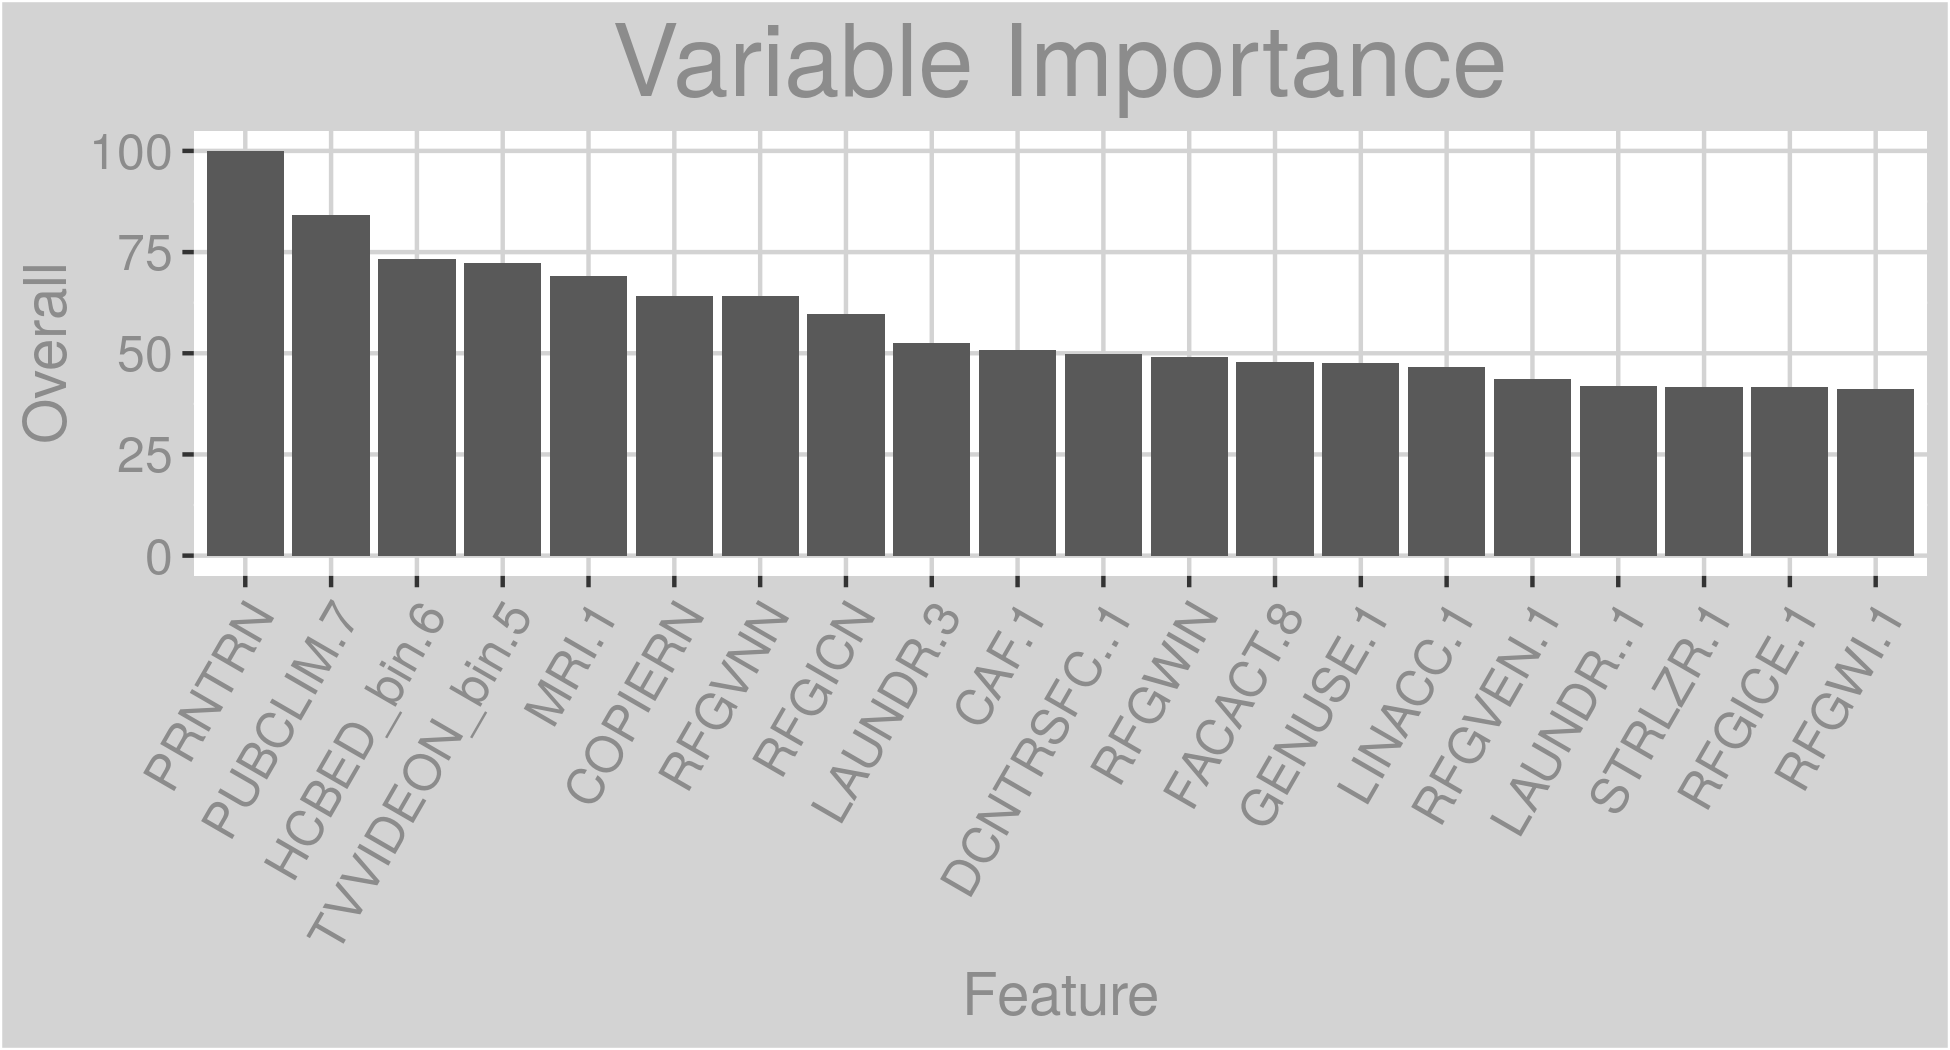
\includegraphics[width=.99\textwidth, height=0.35\textheight]{Images/electricity_all_vars.png}
\\[0.2in]
In order to rank the most important features, the variable importance metrics from the selected models were all set to the same scale, the summed up.  The number of selected features were then used as hyperparameters in the final model training.  As a preliminary check, the top 20 predictors are plotted in the appendix and are generally discussed here.  It seems the attempts to create stratified random samples, by building type, may have been beneficial in this case since there are some very building type specific end-uses that are highly ranked.  It does cause some concern that there are some odd selections, such as the 'witheld' column of the climate encoded variables being selected; however, it seems as though whatever reasoning to classify these types of buidlings this way is a direct indicator of electrical consumption.  When evaluating multiple selected atypical variables (e.g. LAUNDR.3[laundry provided by offsite services]) it seems that just the applicability of the question influences the consumption (building types - lodgining, healthcare, nursing).  In an attempt to truly follow the imporant predictors, no variables have been removed from this set and the order of importance remains unchanged.